
% \maketitle \Large

\chapter{A note on the theory of rent and urban economic development, August 22 2022}

\epigraph{ Alonso's model has become the standard tool for understanding urban economics. Because it incorporates land rent explicitly, it can provide the foundation for a  formal analytical approach to the distribution of  the surplus generated by an urban system.}

\section{initial notes}
This document describes the link between housing cost, rent theory, and urban prosperity. The analysis has important implications for Ontario Housing Policy and Canadian economic development

The key idea is that cities are productive - they generate a surplus over and above the labour and resources that go into them. We want to understand how the surplus wealth produced by cities is distributed and how it affects the economy.  

It turns out that ownership of land determines  who gets the surplus. Land is a natural resource -- no one creates it. The share or production that goes to landowners is called "rent." To  understand what is happening in our cities we need a basic grasp of  rent theory. To provide that basic understanding, we first very briefly review the familiar supply and demand graph, then show how rent theory is implicit in the model when we apply it to  the ownership of agricultural land. That allows us to show how the basic model of modern urban economic is a variant of Ricardo's model and can be used to approach the question of distribution. Finally we examine some policy implications that follow from the application of rent theory to the current housing crisis.

\section{A preamble}
In 1817 David Ricardo provided the basic economic explanation for the wealth and power of the landowning classes in Britain. Ricardo's insights remain  standard tools of modern economics, although submerged in every first year economics course as consumer and producer surplus, in urban theory as the classic urban rent profile and in institutional theory as  "rent seeking."

Straightforward application of Ricardo's insight using simple supply and demand curves allows us to understand the current housing crisis and the national productivity crisis. It also points the way to a strategy that can solve the housing crisis, make Canadians better off and increase the productivity of the Canadian economy.


\begin{figure}[htbp]
\begin{center}
  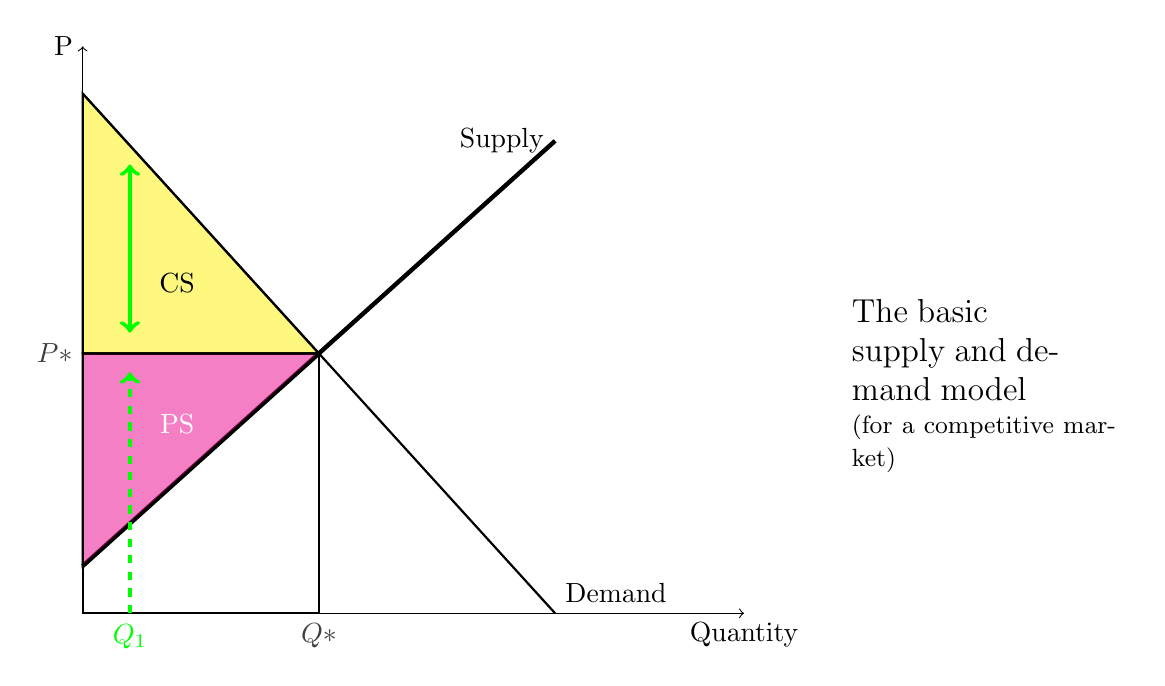
\begin{tikzpicture}[domain=0:2,scale=1.2]        %NINE panesl Top lcr M lcr Blcr
%%%%%%%%%%% 								               TOP%%%     
 %	 \begin{scope}[scale=.6, shift={(6,20.5)}]  % Tr : features of S and D 
			%  \draw [gray] (0,0) grid (7,7);
		\draw [<->] (0,6)node[left]{P} -- (0,0) -- (7,0)node[below]{Quantity};
  
		\draw [thick] (0,5.5) -- (5,0)node[above right]{Demand};
	%	\node at (5,0)[below]{$Q_{max}$};
		\draw [ultra thick] (0,.5) -- (5,5)node[left]{Supply};
				 
		 \draw [thick, fill opacity=0.75] % fill=yellow,
		 		(0,0) -- (0,2.75) node[left]{$P*$}--(2.5, 2.75) --(2.5, 0)node[below]{$Q*$} -- cycle;
 		\draw [thick, fill=yellow, fill opacity=0.5]  
				(0,5.5) -- (0,2.75) --(2.5, 2.75) -- cycle;
 		\draw [thick, fill=magenta, fill opacity=0.5]  
				(0,.5) -- (0,2.75) --(2.5, 2.75) -- cycle;

		 \node at (1,2) (b) [white] {PS};
		  \node at (1,3.5) (b) [black] {CS};

	\draw [ultra thick, green, <->] (.5, 4.75) -- (.5, 2.97);
	\draw [dashed, ultra thick, green, ->] (.5, 0)node[below]{$Q_1$} -- (.5, 2.55);

  \begin{scope}[scale=.6, shift={(10,0)}] 
		    \node at (6,4) (b) [black, text width=3.5cm] {\large The basic \\supply and demand model\\ {\small (for a competitive market)}};
\end{scope}		    
\end{tikzpicture}
\caption{The basic supply and demand graph}
\label{fig:city_supply_and_demand}
\end{center}
\end{figure}

\section{Basic Supply and Demand}
Although the basic supply and demand graph had not been invented in Ricardo's time, we can use it to illustrate the Ricardo's insights. In Figure~\ref{fig:city_supply_and_demand}, the height of the demand curve at each quantity represents how much buyers will pay for  one more unit of whatever is being sold in this market. The height of the supply curve is the cost of producing one more unit. Producers won't want to sell any units that cost more than they are being paid.

To read the graph, we can pick a price, and read horizontally to the demand curve to `predict' how many  consumers  want to buy at that price, and across  the supply curve to find out how many producers want to sell. If they don't agree on a quantity to transact, we say ``the market doesn't clear.''  At the price $P*$, where the curves cross, however, they will agree on quantity, so we'll assume the this becomes the market price.

The graph doesn't just describe buyer and seller behaviour leading to a market price and quantity. It can also measure the social benefits produced by the private market. Some  buyers would have bought the product even at a price higher than the market price. The difference  between the price they pay and the the price they were wiling to pay is an \textbf{economic surplus}.  The solid green arrow in the yellow area of the figure is the amount of this excess benefit called   `consumer surplus' received by whoever bought unit $Q_1$. The yellow area is the sum of consumer surplus of all buyers. 

Similarly, the magenta area below the price line is what economists call "\textbf{producer surplus}" -- the difference between the sale price and the \textbf{marginal} cost of production. It is not profit because most producers still have to pay the costs of producing capital goods. Fixed costs have to be deducted. 


%Overall, the supply and demand graph  is a remarkably simple  model that lets us think clearly  the behaviour of hundreds, or even millions, of two different kinds of people, the buyers and sellers, when they interact. It finds a combination of price and quantity that is likely to be reasonably stable, and it can be applied to all kinds of markets. 

\section{Ricardo's problem}
In agriculture the cost of producing land is zero. Land is a "free gift of nature''. As a result, agriculture in the entire producer surplus is available to distribute. Ricardo didn't call it producer surplus, however. That term had not been invented. He used a term that was already applied to the agricultural surplus: \textbf{rent}.

 Ricardo's theory  explained how the surplus produced by the land was shared between landowners and labour. We can adapt the supply and demand  model to describe what Ricardo discovered.  

 
\begin{figure}[htbp]
\begin{center}

  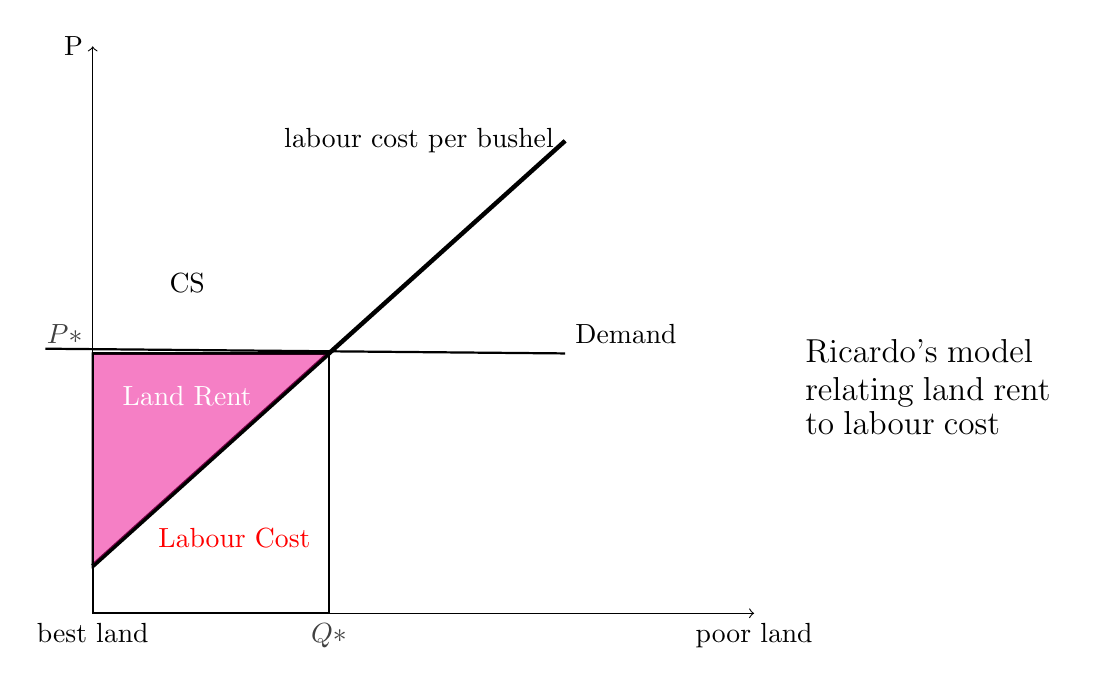
\begin{tikzpicture}[domain=0:2,scale=1.2]        %NINE panesl Top lcr M lcr Blcr
%%%%%%%%%%% 								               TOP%%%     
 %	 \begin{scope}[scale=.6, shift={(6,20.5)}]  % Tr : features of S and D 
			%  \draw [gray] (0,0) grid (7,7);
		\draw [<->] (0,6)node[left]{P} -- (0,0)node[below]{best land} -- (7,0)node[below]{poor land};
  
		\draw [thick] (-.5,2.8) -- (5,2.75)node[above right]{Demand};
		%\node at (5,0)[below]{$Q_{max}$};
		\draw [ultra thick] (0,.5) -- (5,5)node[left]{ \normalsize  labour cost per bushel};
				 
		 \draw [thick, fill opacity=0.75] % fill=yellow,
		 		(0,0) -- (0,2.75) node[above left]{$P*$}--(2.5, 2.75) --(2.5, 0)node[below]{$Q*$} -- cycle;
 	%	\draw [thick, fill=yellow, fill opacity=0.5]  
				(0,5.5) -- (0,2.75) --(2.5, 2.75) -- cycle;
 		\draw [thick, fill=magenta, fill opacity=0.5]  
				(0,.5) -- (0,2.75) --(2.5, 2.75) -- cycle;
				
 		 \node at (1.5,.8)  (a) [red] { \normalsize Labour Cost};
		 \node at (1,2.3) (b) [white] { \normalsize Land Rent};
		  \node at (1,3.5) (b) [black] {CS};

	%\draw [thick,dashed] (.5,7) -- (.5,0)node[below]{$Q_{low}$};


  \begin{scope}[scale=.6, shift={(10,0)}] 
		    \node at (5,4) (b) [black, text width=3.5cm] {\large Ricardo's 
model\\ relating land rent\\ to labour
cost};
\end{scope}		    
\end{tikzpicture}
\caption{Ricardo's Figure}
\label{Fig:Ricardo'sFigure}
\end{center}
\end{figure}


 In Figure~\ref{Fig:Ricardo'sFigure}, the height of the supply curve from Figure~\ref{fig:city_supply_and_demand}   becomes the labour cost of producing  `corn' (we call it wheat now) on each plot of land, from best on the left to the worst on the right. Naturally cost in labour rises as we move to less productive. The supply curve now shows the rising cost as more land is planted.
 
 Since Ricardo was  just dealing with the production side and assuming that landowner and peasant knew roughly what  price would be paid for `corn' (we call it wheat now), we can  draw the demand curve for  Figure~\ref{Fig:Ricardo'sFigure} as a horizontal line and w e can ignore consumer surplus.

Landowners didn't actually farm, and they didn't usually hire workers to farm the way that an industrial capitalist did. They rented plots land to peasant farmers.  Maximizing their rent  income meant minimizing the share of the surplus that the peasants got to keep. Since land was scarce and peasants were numerous, the landlord generally had the upper hand and could squeeze out something close to the maximum rent.\footnote{After the black death there were fewer peasants  and they were able to negotiate lower rents}. Peasants got paid for their labour, often just a subsistence wage, and landowners captured all of the surplus in Ricardo's theory.

%Landowner and peasant knew roughly what  price would be paid for `corn' (we call it wheat now) when it was produced, how much corn a particular plot would produce, and how much work it would take to produce that corn. Although the rent-setting process was probably quite different, we can imagine the peasant knowing the maximum he would bid to farm a particular lot.  We can imagine the peasant and the landlord negotiating over the rent. 

\section{Modern Urban Economics}
Bid rent theory\footnote{Location and Land Use, (1964) by William Alonso.} is a geographical economic theory that refers to how the price and demand for real estate change as the distance from the central business district (CBD) increases.\footnote{von Th\"unen's The Isolated State (1826) generates a pattern of agricultural land use based on transportation costs and can be seen as synthesizing Alonso and Ricardo's insights. } It is essentially Ricardo's rent theory, except that the figure is turned upside down and labour cost  is replaced with transportation cost, as in Figure~\ref{Fig:Alonso'sFigure}. 

In this model, workers demand land that provides access to wage employment at the core. Their willingness to pay -- their bid rent -- is lower for land farther from the core because the transportation costs eat up some of the wage. 

As in Ricardo's model, landowners capture the land rent.  Urban tenants are in the same position as Ricardo's tenant farmers with respect to land rents. Like freehold farmers, owner occupiers capture the land rent  for their own property.


\begin{figure}[htbp]
\begin{center}

  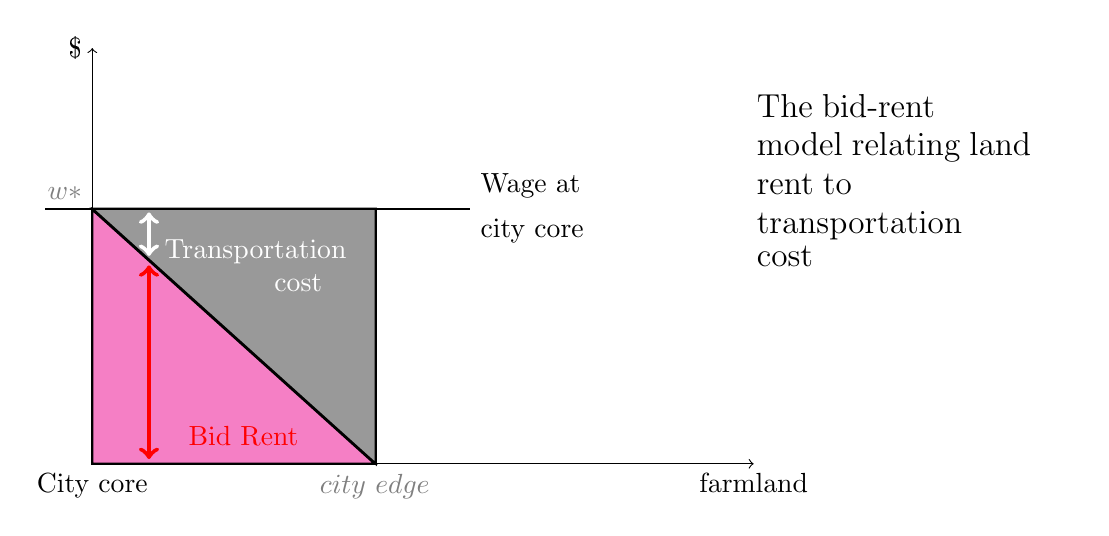
\begin{tikzpicture}[domain=0:2,scale=1.2]        %NINE panesl Top lcr M lcr Blcr
%%%%%%%%%%% 								               TOP%%%     
 %	 \begin{scope}[scale=.6, shift={(6,20.5)}]  % Tr : features of S and D 
			%  \draw [gray] (0,0) grid (7,7);
\draw [<->] (0,4.4)node[left]{\$} -- (0,0)node[below]{City core} -- (7,0)node[below]{farmland};
\draw [thick] (-.5,2.7) -- (4,2.7)node[above right]{Wage at}node[below right]{city core};
				 
 \draw [thick, fill=magenta, fill opacity=.5] 	(0,0) -- (0,2.69) node[above left]{$w*$}--(2.99, 0)node[below]{$city\ edge$} -- cycle;
\draw [thick, fill=black, fill opacity=0.4]  (0,2.7) -- (3,0) --(3, 2.7) -- cycle;
				
\node at (1.6,.3)  (a) [red] { \normalsize Bid Rent};
 \node at (1.6,2.1) (b) [white, text width=2cm, align = right ] { \normalsize Transportation cost};

\draw [ultra thick, white,< ->]    (.6, 2.2)-- (.6, 2.66);	
\draw [ultra thick, red, <->] (.6, .05) -- (.6, 2.1);



  \begin{scope}[scale=.6, shift={(10,0)}] 
		    \node at (4.5,5) (b) [black, text width=4cm] {\large The bid-rent \\model relating land  rent to \\transportation\\ cost\normalsize};
\end{scope}		    
\end{tikzpicture}
\caption{The bid-rent model}
\label{Fig:Alonso'sFigure}
\end{center}
\end{figure}
 Alonso's model has become the standard way  of understanding urban economics. Because it incorporates land rent explicitly, it it can provide the foundation for a  formal analytical approach to the distribution of  the surplus generated generated by an urban system.
  

